\section{Physic's Model Study}
The haptic device we developed for this thesis is at its heart a \textbf{multi-physical system}, where electrical, magnetic, and mechanical components interact with each other.
Voice coil actuators are characterized by three main components: a \textbf{coil}, a \textbf{magnet}, and a \textbf{membrane}. The coil generates a magnetic field when a \textbf{current flows} through it and by interacting with the magnetic field generated by the magnet, \textbf{creates a force} that moves the membrane. The membrane is then used to \textbf{transmit this force} to the user's finger, which can feel the force as a \textbf{vibration}.
In this section, we will try to create a complete model to explain its behavior using \textbf{bond graphs}.
\begin{figure}[H]
    \centering
    \resizebox{1\linewidth}{!}{
        \begin{tikzpicture}
    \begin{scope}[every node/.style={bgelement}]
    \node (Se) at (0,0) {Se: Power Supply};
    \node[right=1 of Se] (i) {1: elec};
    \node[above=1 of i] (Iel) {I: L\textsubscript{coil}};
    \node[below=1 of i] (Rel) {R: R\textsubscript{coil}};
    \node[right=1 of i] (CI) {CI: Coil+Magnet};
    \node[right=1 of CI] (w1) {1: mech};
    \node[above=1 of w1] (Cm) {C: C\textsubscript{membrane}};
    \node[below=1 of w1] (Im) {I: M\textsubscript{magnet} + M\textsubscript{finger}};
    \node[right=1 of w1] (v) {0};
    \node[above=1 of v] (w2) {1};
    \node[above=1 of w2] (Rdf) {R: Rd\textsubscript{finger}};
    \node[right=1 of w2] (Cf) {C: $\frac{1}{Ks_{finger}}$};
    \node[right=1 of v] (Sfa) {S\textsubscript{finger}};
    \end{scope}
    \draw[bonds]
    (Se) edge [e_out] (i)
    (i) edge [e_in] (Iel)
    edge [e_in] (Rel)
    edge [e_in] (CI)
    (CI) edge [e_in] (w1)
    (w1) edge [e_out] (Cm)
    edge [e_in] (Im)
    (w1) edge [e_in] (v)
    (v) edge [e_in] (w2)
    (w2) edge [e_in] (Rdf)
    (w2) edge [e_in] (Cf)
    (Sfa) edge [e_out] (v);
\end{tikzpicture}
    
    } % TODO: Da fare bene
    \caption{Bond graph of the entire system, including the finger.}
    \label{fig: Total_bond-graph}
\end{figure}

\subsection{Electrical and Power Aspects of Coils}
The electrical part consists of the \textbf{voltage power supply} and the coil which is modeled as a \textbf{resistor} and an \textbf{inductor} in series. For this research, we're using planar concentric coils built using \textbf{flexible PCB technology}, this allows us freedom of design in creating a \textbf{flexible actuator}.
Due to their nature, these coils are very thin, which results in \textbf{high resistance} and \textbf{high heat production}. The power flowing through the coil must be \textbf{kept low to avoid damaging it}. This in turn means that the magnetic field generated by the coil will be \textbf{weak}, which introduces challenges when trying to create strong haptic feedback.

\subsection{Electro-mechanical Transducer}
The electrical energy is converted into mechanical motion through the \textbf{magnetic repulsion} between the coil and magnet, so the system acts as a \textbf{transducer}.
\begin{figure}[H]
    \centering
    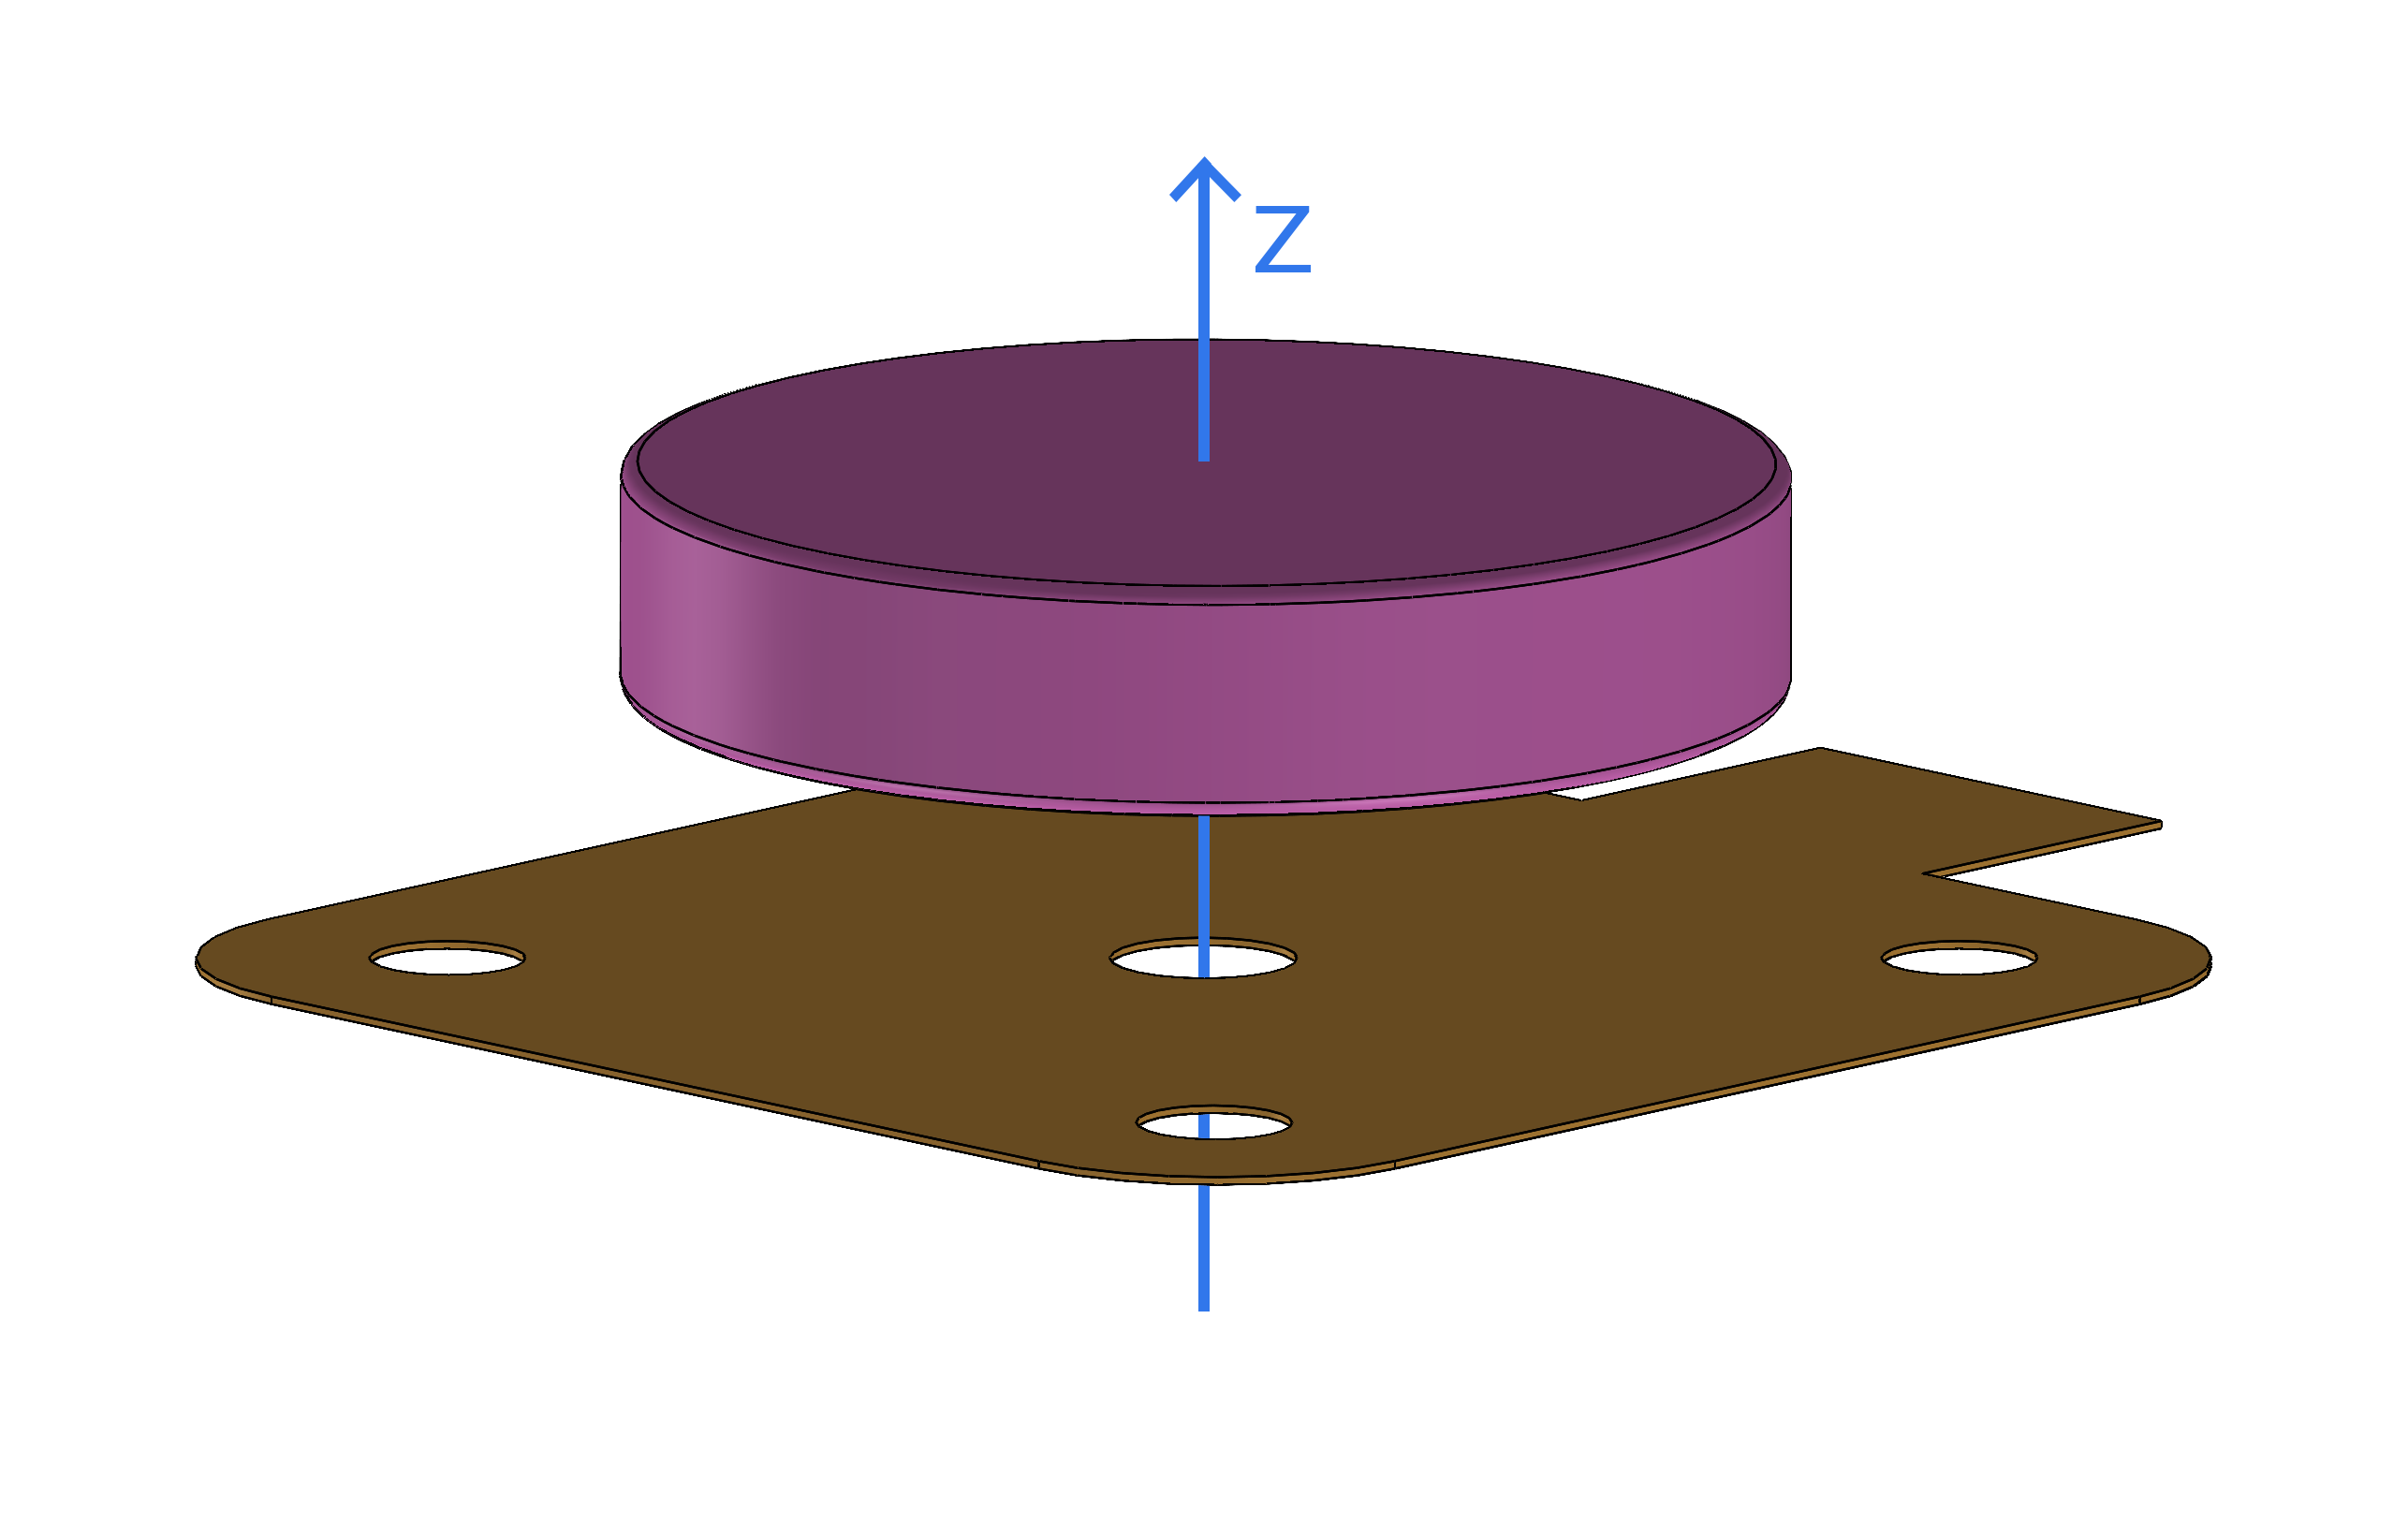
\includegraphics[width=0.4\columnwidth]{Figures/coil_magnet.png} 
    \caption[Coil-Magnet position]{Coil and magnet position in space.}
\end{figure}
The force is calculated through the \textbf{magnetic levitation} equation between the magnetic moment of the magnet and the magnetic field generated by planar windings:
\begin{equation*}
    F = \nabla (\overrightarrow{m_M} \cdot \overrightarrow{B_C}) = \frac{d}{dz} \left( \frac{B_M(z)}{\mu} \cdot \frac{\mu N I R_C^2}{2(R_C^2+z^2)^\frac{3}{2}} \right)
\end{equation*}

\subsection{Mechanical Membrane}
To limit the motion of the magnet only to the z-axis the magnet is inserted in a \textbf{flexible membrane}, this membrane is also used to \textbf{transmit the force} generated by the magnet to the user's finger.
For the last prototype, we designed a \textbf{celtic-cross-shaped silicone membrane} where the magnet is inserted in the center of the cross.
\begin{figure}[H]
    \centering
    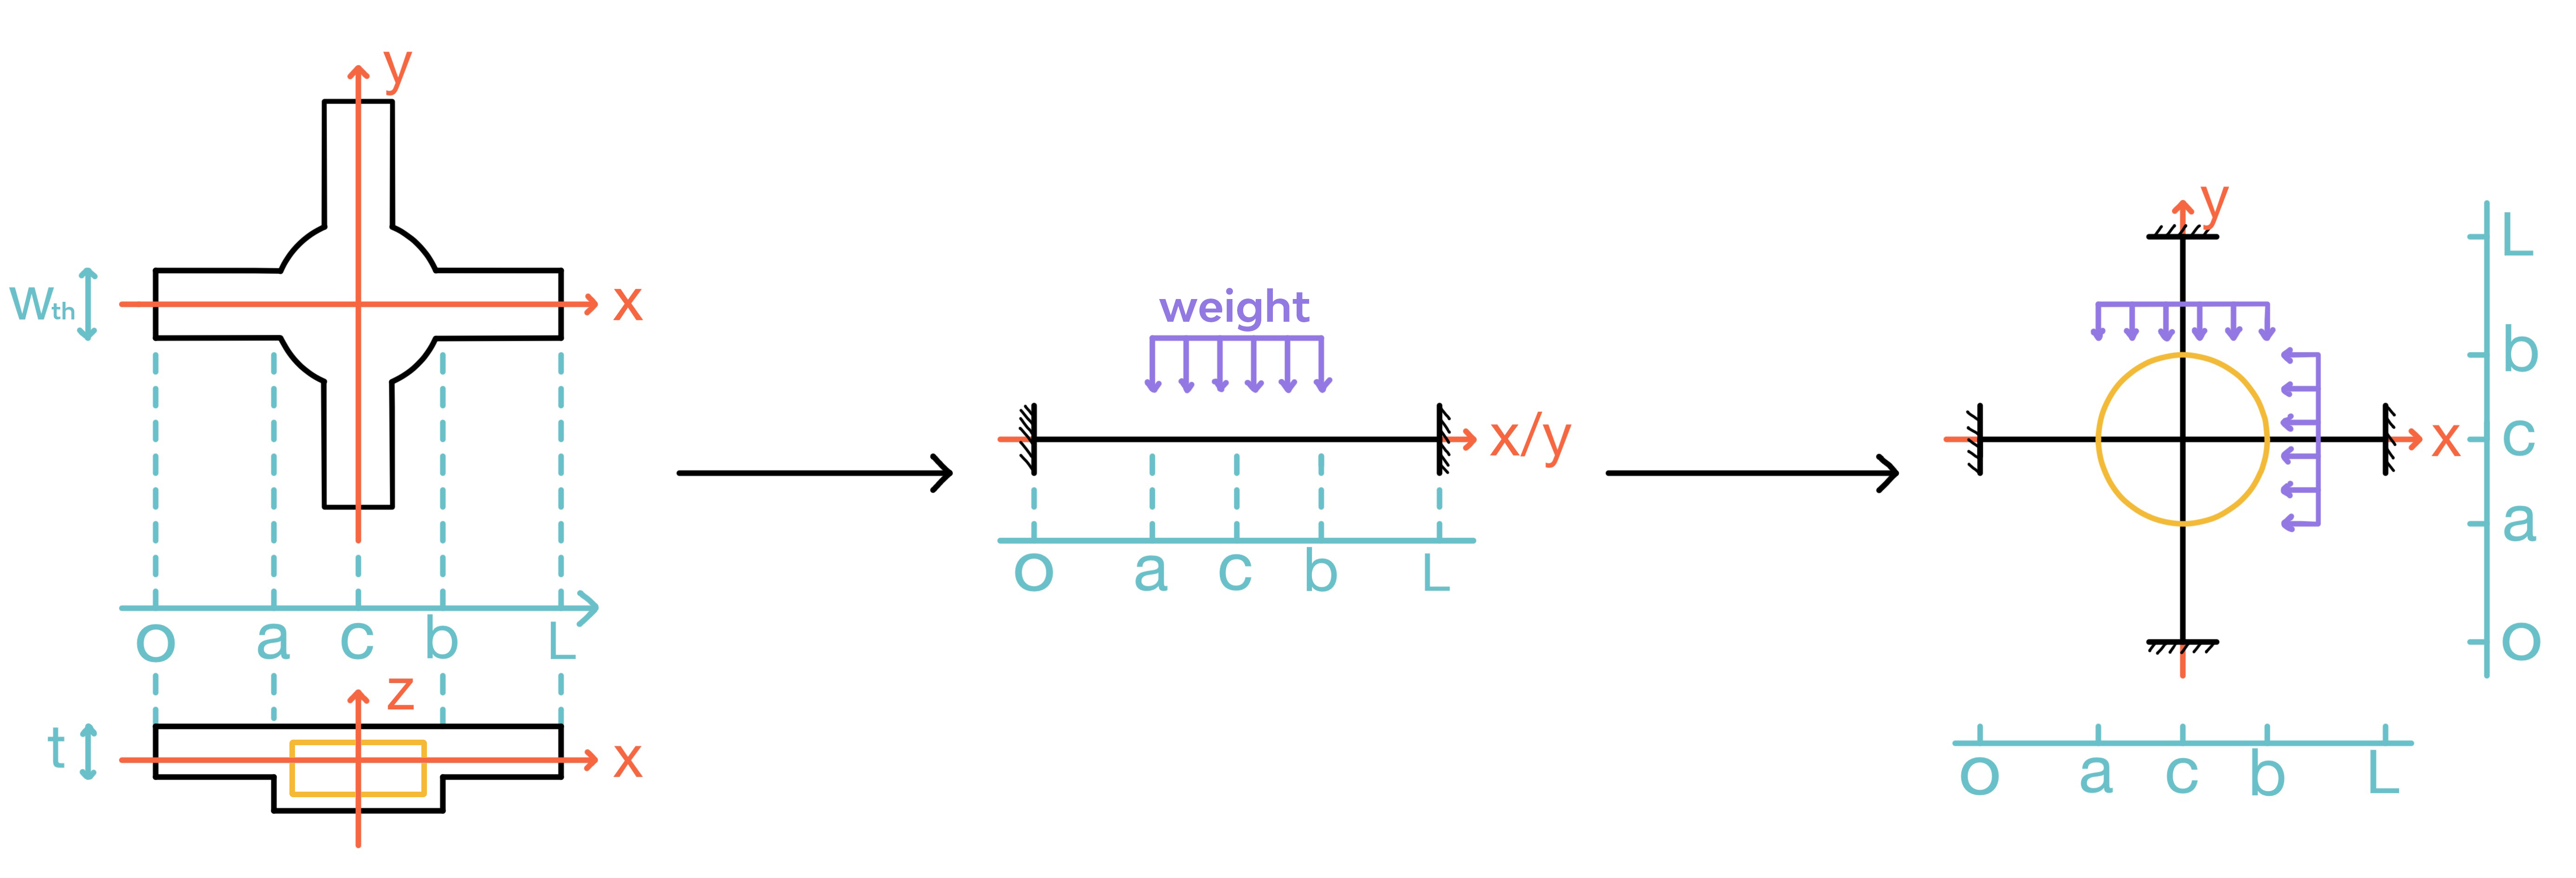
\includegraphics[width=0.9\linewidth]{Figures/membr_mech_model.jpg} 
    \caption[Membrane structure]{Membrane's structure and mechanical model.}
\end{figure}
The membrane can be modeled as a \textbf{spring-damper system}, where the spring represents the stiffness of the membrane, and the damping is negligible.
Finally, the finger grasping the membrane can also be modeled as a \textbf{mass-spring-damper} system where the inertia component is represented by the finger's mass, while the spring and damper represent respectively the stiffness and damping effects of the finger's skin.
